\documentclass{beamer}

\mode<presentation> {


\usetheme{Boadilla}

\usecolortheme{whale}

%\setbeamertemplate{footline} % To remove the footer line in all slides uncomment this line
%\setbeamertemplate{footline}[page number] % To replace the footer line in all slides with a simple slide count uncomment this line

\setbeamertemplate{navigation symbols}{} % To remove the navigation symbols from the bottom of all slides uncomment this line
}

\usepackage{amsmath,amsfonts,amssymb}
\usepackage{graphicx}
\usepackage{booktabs}
\usepackage{lmodern}
\usepackage{animate}
\usepackage{IEEEtrantools}
\usepackage{multicol,multirow}
% \usepackage{biblatex}

%----------------------------------------------------------------------------------------
%	TITLE PAGE
%----------------------------------------------------------------------------------------

\title[Decomposing Assembly Lines]{A Hybrid Benders Decomposition of the Assembly Line}


\author{Kenneth D. Young}
\institute[UniMelb]
{
AMSI Optimise Workshop\\[2mm]
Masters Thesis\\[2mm]
Supervisor: Dr. Alysson M. Costa\\
}
\date{$29^{\text{th}}$ of June, 2017}

\begin{document}

\begin{frame}
\titlepage
\end{frame}

%------------------------------------------------
\begin{frame}
\frametitle{Overview}
\begin{enumerate}
	\item The Problem: Assembly Line Balancing \vspace{1cm}
	\item The Method: Benders Decomposition \vspace{1cm}
	\item Results
\end{enumerate}
\end{frame}

%------------------------------------------------
\begin{frame}
\frametitle{Assembly Lines through History}
% \vspace{-0cm}
\begin{figure}
	\centering
	\begin{minipage}{0.47\textwidth}
		\centering
		Ford Motor Company, Detroit 1915\\[2mm]
		\includegraphics[width=\linewidth]{images/history-1.jpg}
	\end{minipage}
	\hspace{2mm}
	\begin{minipage}{0.45\textwidth}
		\centering
		Volkswagen, Wolfsburg 1951\\[2mm]
		\includegraphics[width=\linewidth]{images/history-5.jpg}
	\end{minipage}
\end{figure}
% \vspace{-5cm}
% \begin{figure}
% 	\centering
% 	\includegraphics[width=0.6\linewidth]{images/history-4.jpg}\\
% 	Honda, Ontario 2012
% \end{figure}
% \vspace{-5cm}
% \tiny
% Photos distributed under the CC-BY 2.0 license
\end{frame}

%------------------------------------------------
\begin{frame}
\frametitle{Assembly Lines through History}
\centering
Kia Motors, \v{Z}ilina 2012\\[2mm]
\animategraphics[loop,controls,height=0.7\textheight]{12}{images/kia-}{0}{66}

% \tiny
% Photos distributed under the CC-BY 2.0 license
\end{frame}

%------------------------------------------------
\begin{frame}
\frametitle{The Assembly Line Balancing Problem}
Production system designed to \emph{efficiently} manufacture a product\vspace{3mm}\pause	
\begin{enumerate}
	\item Tasks \vspace{2mm}
	\item Work stations\vspace{2mm}
	\item Precedence Relations\pause
\end{enumerate}
\vspace{4mm}
$Def^{\underline{n}}$: The {\color{red} cycle time} of the line is
the largest workload among all stations
\[ c = \max\{\: l_k \: | \: k\in K\:\} \]
	where $K$ is the set of stations and $l_k$ is the load of station $k$
\end{frame}

%------------------------------------------------
\begin{frame}
\frametitle{The Type-2 ALBP}
\begin{itemize}
	\item Two main kinds of assembly line problems: Type-1 and Type-2.\vspace{3mm}\pause\\
	\item We consider the Type-2 case:\vspace{2mm}
	\begin{itemize}
		\item Fixed number of work stations\vspace{1mm}
		\item Variable cycle time\vspace{3mm}\pause
	\end{itemize}
	\item 
	{\color{red} Aim:} Maximize production rate $\iff$ Minimize cycle time\vspace{2mm}
	\begin{itemize}
		\item By balancing workload across the stations\vspace{3mm}\pause
	\end{itemize}
	\item What are our decisions?\vspace{2mm}
	\begin{itemize}
		\item Assigning tasks to stations
	\end{itemize}
\end{itemize}
% \vspace{3mm}
% Constraints:
% \vspace{2mm}
% \begin{itemize}
% 	\item Precedence Relations
% \end{itemize}
\end{frame}

%------------------------------------------------
\begin{frame}
\frametitle{Simple Assembly Line Example}
\begin{overlayarea}{\textwidth}{\textheight}
\begin{figure}
	\centering
	\hspace{5mm}%
	\begin{minipage}{0.3\textwidth}%
		\centering%
		4 Tasks\\[2mm]%
		3 Stations%
	\end{minipage}%
	\hfill%
	\begin{minipage}{0.6\textwidth}%
		\centering%
			\only<1>{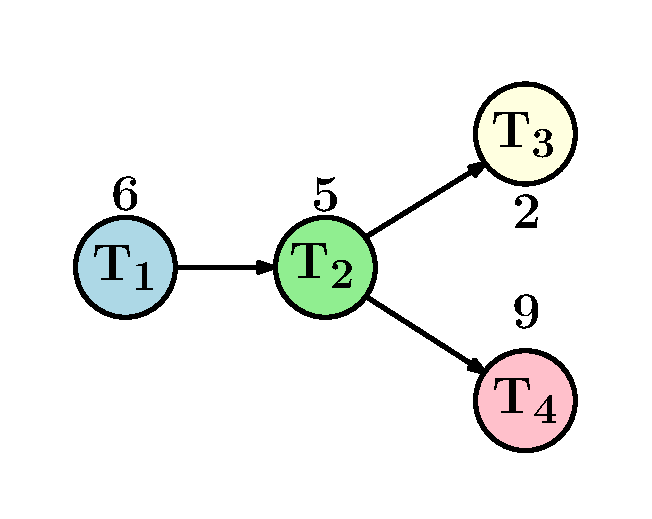
\includegraphics[height=0.3\textheight]{images/precgraphStations-1.eps}}%
			\only<2>{\includegraphics[height=0.3\textheight]{images/precgraphStations-2.eps}}%
			\only<3>{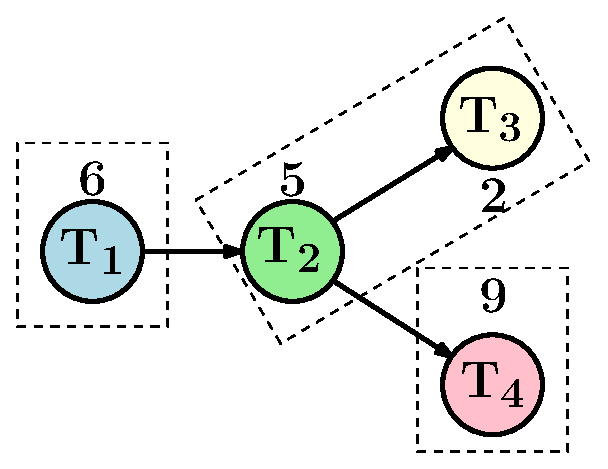
\includegraphics[height=0.3\textheight]{images/precgraphStations-3.eps}}%
	\end{minipage}%
\end{figure}%
\vspace{-1cm}%
\begin{figure}%
	\centering%
	\only<1>{
\includegraphics[width=0.45\textwidth]{images/exSimpleBlank.eps}}%
	\only<2>{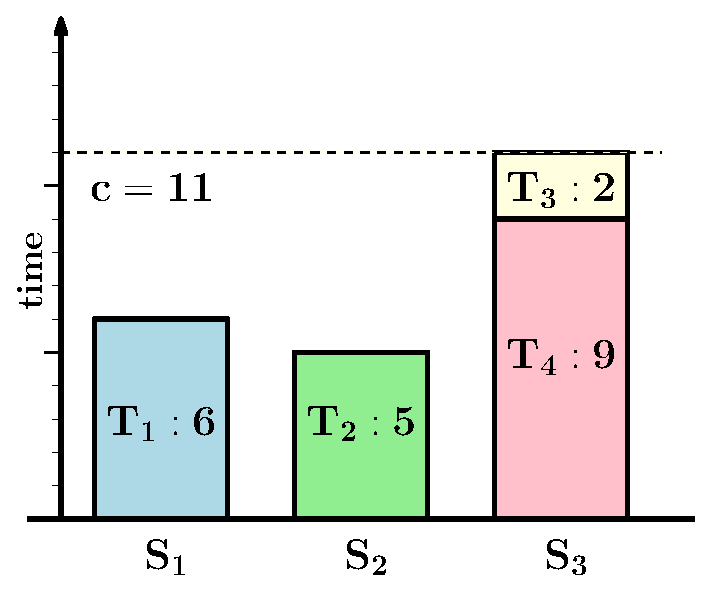
\includegraphics[width=0.45\textwidth]{images/exSimpleFeas.eps}}%
	\only<3>{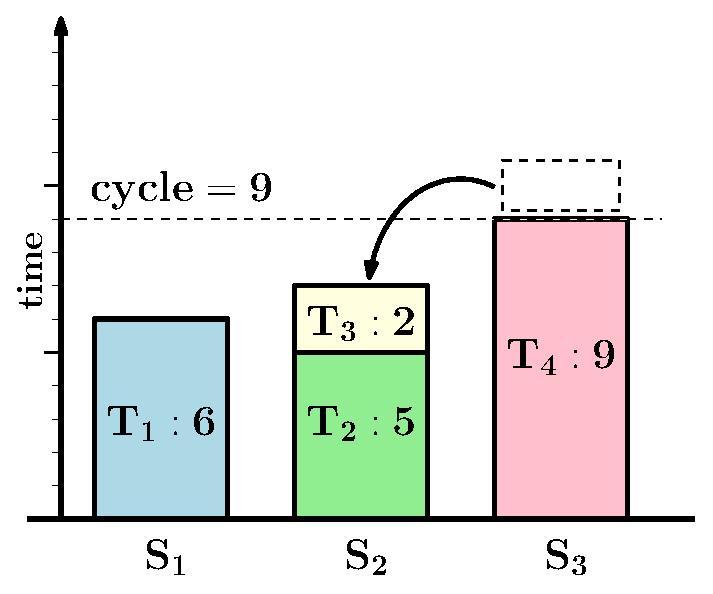
\includegraphics[width=0.45\textwidth]{images/exSimpleOpt.eps}}%
\end{figure}%
\end{overlayarea}
\end{frame}

%------------------------------------------------
\begin{frame}
\frametitle{Sequence-Dependent Setup Times}
\begin{itemize}
	\item Theory usually assumes task sequence within a station can be arbitrary\vspace{2mm}
	\begin{itemize}
		\item Not always the case in practice!\vspace{2mm}\pause
	\end{itemize}
	\item Setup times between tasks can vary a lot\vspace{2mm}
	\begin{itemize}
		\item Walking distances\vspace{1mm}
		\item Tool-changes (esp. in robotic assembly lines)\vspace{1mm}
		\item Cooling periods\vspace{3mm}\pause
	\end{itemize}
	\item Considering setups leads to the SetUp Assembly Line Balancing and Scheduling Problem, or SUALBSP\vspace{1mm}
	\begin{itemize}
		\item Type-2 problem is denoted SUALBSP-2
	\end{itemize}
\end{itemize}
\end{frame}

%------------------------------------------------
\begin{frame}
\frametitle{The SUALBSP-2}
\begin{itemize}
	\item SUALBSP-2 can be viewed as $m$ Travelling Salesperson Problems where the set of cities for each TSP is unknown\vspace{3mm}\pause
	\item Two distinct types of setups/distances between tasks/cities\vspace{1mm}
	\begin{itemize}
		\item $\phi_{ij}=$ Forward setup between tasks on same product\vspace{1mm}
		\item $\beta_{ij}=$ Backward setup between last task on product $p$ and first task on $p+1$\vspace{2mm}\pause
	\end{itemize}
	\item Consider one station with tasks $T_i$, $T_j$ and $T_k$:
\end{itemize}

\begin{figure}
	\centering
	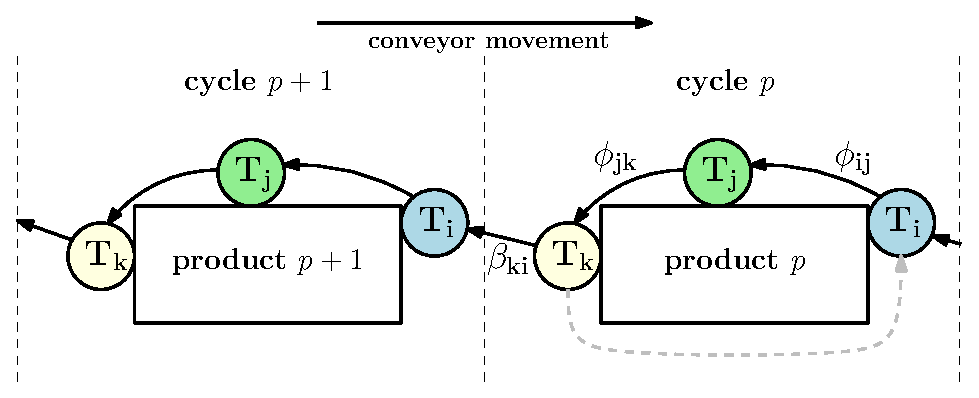
\includegraphics[width=0.8\textwidth]{images/IntroForwBackSetupEx.eps}
\end{figure}
\end{frame}

%------------------------------------------------
\begin{frame}
\frametitle{Example with Setup Times}
\begin{table}
	\centering
	\begin{minipage}{0.15\textwidth}
		\centering
		\only<1>{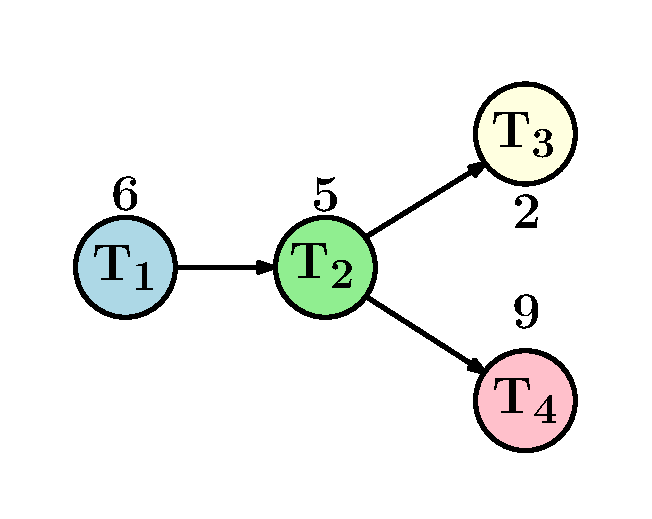
\includegraphics[width=\linewidth]{images/precgraphStations-1.eps}}%
		\only<2>{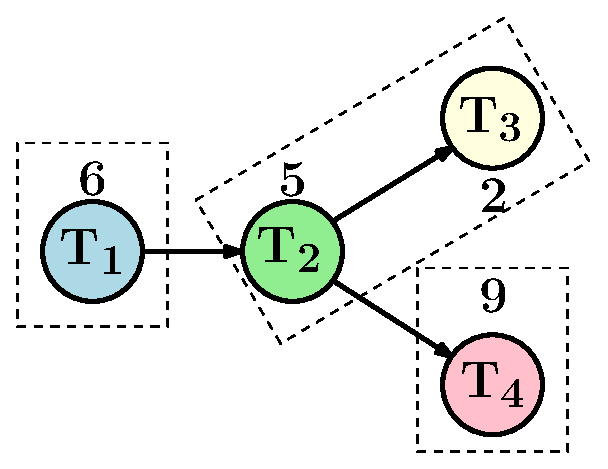
\includegraphics[width=\linewidth]{images/precgraphStations-3.eps}}%
		\only<3>{\includegraphics[width=\linewidth]{images/precgraphStations-2.eps}}%
	\end{minipage}
	\hspace{0mm}
	\begin{minipage}{0.3\textwidth}
		\centering
		\begin{tabular}{lllll}
			\toprule
			$\phi_{ij}$ & $T_1$ & $T_2$ & $T_3$ & $T_4$ \\\midrule
			$T_1$ & -- & 3 & 3 & 3 \\
			$T_2$ & -- & -- & 2 & 3 \\
			$T_3$ & -- & -- & -- & 1 \\
			$T_4$ & -- & -- & 2 & -- \\
			\bottomrule
		\end{tabular}
	\end{minipage}
	\hspace{10mm}
	\begin{minipage}{0.3\textwidth}
		\centering
		\begin{tabular}{lllll}
			\toprule
			$\beta_{ij}$ & $T_1$ & $T_2$ & $T_3$ & $T_4$ \\\midrule
			$T_1$ & 0 & -- & -- & -- \\
			$T_2$ & 3 & 0 & -- & -- \\
			$T_3$ & 3 & 5 & 0 & 3 \\
			$T_4$ & 3 & 3 & 1 & 0 \\
			\bottomrule
		\end{tabular}
	\end{minipage}
\end{table}
\pause
\begin{figure}
	\centering
	\only<1>{
\includegraphics[width=0.45\textwidth]{images/exSimpleBlank.eps}}%
	\only<2>{\includegraphics[width=0.45\textwidth]{images/exSimpleSetupFeas.eps}}%
	\only<3>{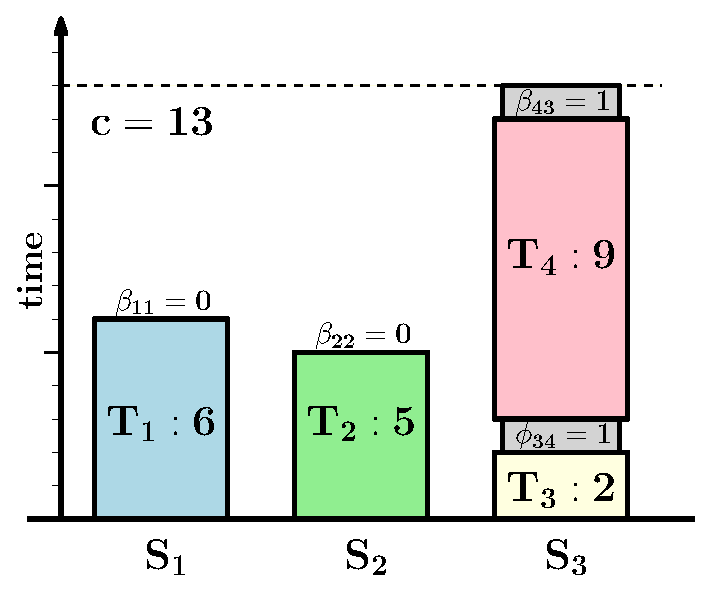
\includegraphics[width=0.45\textwidth]{images/exSimpleSetupOpt.eps}}%
	% \begin{minipage}{0.45\textwidth}
	% 	\centering
	% 	\includegraphics[width=\linewidth]{images/exSimpleSetupFeas.eps}\pause
	% \end{minipage}
	% \hfill
	% \begin{minipage}{0.45\textwidth}
	% 	\centering
	% 	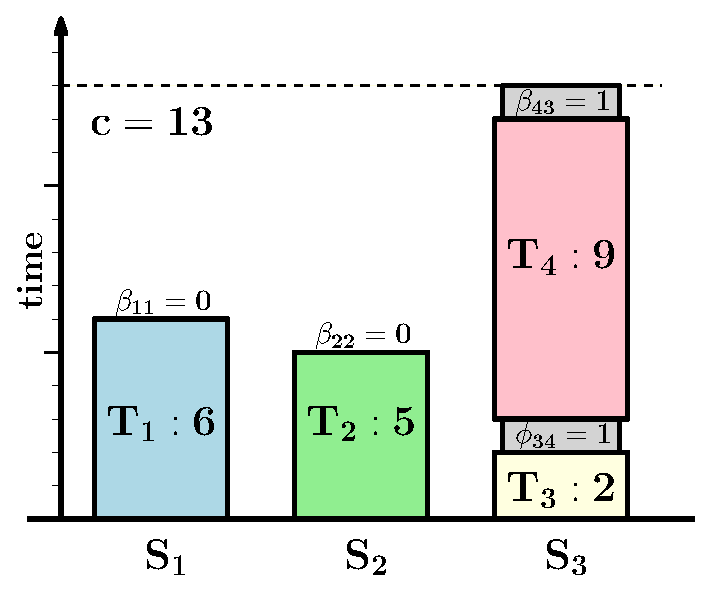
\includegraphics[width=\linewidth]{images/exSimpleSetupOpt.eps}
	% \end{minipage}
\end{figure}
\end{frame}

%------------------------------------------------
\begin{frame}
\Huge{\centerline{Existing Approaches}}
\end{frame}

%------------------------------------------------
\begin{frame}
\frametitle{Data}
\begin{itemize}
	\item Huge data library for ALBPs\vspace{1mm}
	\begin{itemize}
		\item \url{http://assembly-line-balancing.mansci.de/}\vspace{3mm}
	\end{itemize}
	\item 1076 instances of the SUALBSP\vspace{3mm}\pause
	\item We chose 3 subsets with small, medium and large numbers of tasks \vspace{3mm}
	\begin{itemize}
		\item Total of 396 instances\vspace{2mm}\pause
		\item {\color{red} 288 unsolved}\pause
	\end{itemize}
\end{itemize}
\begin{table}
	\centering
	\begin{tabular}{ccccc}
		\toprule
		Data set & \# Instances  & \# Tasks & \# Stations & \# Precedences \\\midrule\midrule
		1 & 108 & 7-21 (small) & 2-8 & 6-27 \\
		2 & 112 & 25-30 (medium) & 3-14 & 32-40 \\
		3 & 176 & 32-58 (large) & 3-31 & 38-62 \\
		\bottomrule
	\end{tabular}
\end{table}
\end{frame}

%------------------------------------------------
\begin{frame}
\frametitle{Exact Solution Procedure}
\begin{figure}
	\centering
	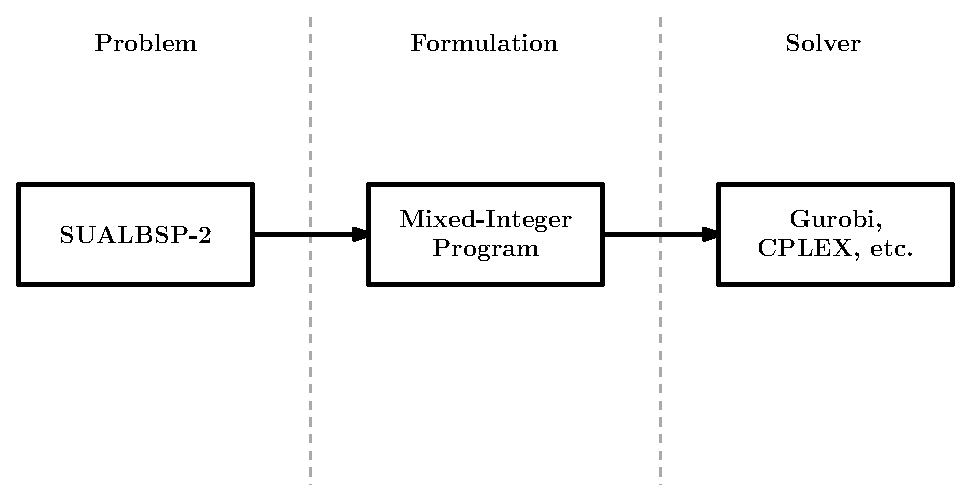
\includegraphics[width=0.95\textwidth]{images/mipApproach.eps}
\end{figure}
\end{frame}

%------------------------------------------------
\begin{frame}
\frametitle{Best Known MIPs for SUALBSP-2}
\pause
\begin{figure}
	\centering
	\begin{minipage}{0.45\textwidth}
		\centering
		\fbox{\includegraphics[width=\linewidth]{images/mip-2.png}}
	\end{minipage}\pause
	\hspace{-2cm}
	\begin{minipage}{0.45\textwidth}
		\centering
		\fbox{\includegraphics[width=\linewidth]{images/mip-1.png}}
	\end{minipage}
\end{figure}
\end{frame}

%------------------------------------------------
\begin{frame}
\frametitle{Results: Mixed Integer Programs}
\begin{itemize}
	% \item 3 data sets: small, medium and large instances\vspace{1mm}
	\item Time limit: 30 minutes for each instance\pause
\end{itemize}
\begin{table}
	\centering
	\begin{tabular}{clrrrrrr}
		\toprule
		\# Tasks & Model & Gap (\%) & No Sol. (\%) & Optimal (\%) & Runtime (s) \\\midrule\midrule
		7--21 & MIP-1 & 0.16 & 0.0 & 93.5 & 166.57 \\
		 & MIP-2 & 1.62 & 0.0 & 86.1 & 374.88 \\\midrule
		25--30 & MIP-1 & 13.76 & 0.0 & {\bf 0.0} & 1800.66 \\
		 & MIP-2  & 18.01 & {\bf 25.0} & {\bf 0.0} & 1800.33 \\\midrule
		32--58 & MIP-1 & 19.56 & 5.1 & {\bf 3.9} & 1759.67 \\
		 & MIP-2 & 10.09 & {\bf 61.9} & {\bf 0.0} & 1800.88 \\
		\bottomrule
	\end{tabular}\pause
\end{table}

``There is a need for more efficient exact methods.''
\begin{flushright}--- Esmaeilbeigi {\it et al.} (2016)\end{flushright}
\end{frame}


%------------------------------------------------
\begin{frame}
\Huge{\centerline{Our Method}}
\end{frame}


%------------------------------------------------
\begin{frame}
\frametitle{Benders Decomposition: History}
\begin{itemize}
	\item Initially proposed by J. F. Benders in 1962\vspace{1mm}
	\begin{itemize}
		\item Created to efficiently solve MIPs\vspace{3mm}\pause
	\end{itemize}
	\item Largely neglected by the literature for $\:\sim40$ years\vspace{3mm}\pause
	\item Recently re-emerged showing it's applicability\vspace{1mm}
	\begin{itemize}
		\item See surveys by Costa (2005) and Rahmaniani \emph{et al.} (2016)\vspace{3mm}\pause
	\end{itemize}
	\item Generalised to \emph{logic-based} Benders decomposition by Hooker (2003)\vspace{1mm}
	\begin{itemize}
		\item Can now be applied to a much wider range of problems
	\end{itemize}
\end{itemize}
\end{frame}

%------------------------------------------------
\begin{frame}
\frametitle{Benders Decomposition: Crash Course}
\begin{itemize}
	\item Strategy: ``learn from your mistakes''\vspace{2mm}\pause
	\item Two types of decisions: {\color{red} primary} and {\color{red} secondary}\vspace{2mm}\pause
	\item Divide the problem into a master problem and a sub-problem \vspace{1mm}
	\begin{itemize}
		\item Iterate between them until optimality
	\end{itemize}
\end{itemize}
\begin{figure}
	\centering
	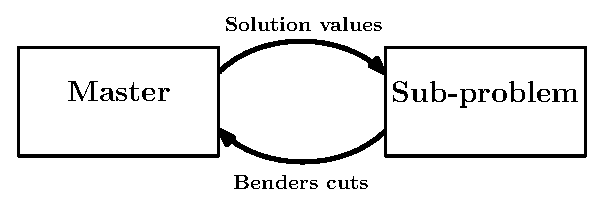
\includegraphics[height=0.3\textheight]{images/bendersAbstract.eps}
\end{figure}\pause
\begin{itemize}
	\item Well-suited to problems with a combinatorial number of constraints\vspace{1mm}
	\begin{itemize}
		\item But only a select few are relevant for finding optimality\vspace{3mm}\pause
	\end{itemize}
	\item Sub-problem tells Master where the most important infeasibilities are
\end{itemize}
\end{frame}

% %------------------------------------------------
% \begin{frame}
% \frametitle{Benders Decomposition: An Example}
% \begin{itemize}
% 	\item Primary variables: $x_1, x_2, x_3$\vspace{2mm}
% 	\item Secondary variables: $y$
% \end{itemize}
% \begin{IEEEeqnarray}{RcRcRcRCl}
% 	\IEEEeqnarraymulticol{9}{c}{\text{Min }~ {\color{black} x_1} ~{\color{black} +~ x_2} ~ {\color{black} +~ x_3} + y }  \nonumber\\[2pt]
% 	\text{subject to }\quad {\color{black} 2 x_1} &\hspace{1mm}&{\color{black} +~x_2} &\hspace{1mm}& &\hspace{1mm}& 3y &\geq& 8  \nonumber\\[2pt]
% 	 &\hspace{1mm}& {\color{black} x_2} &\hspace{1mm}&{\color{black} -~2x_2} &\hspace{1mm}& +~2 y &\geq& 3  \nonumber\\[2pt]
% 	 &\hspace{1mm}& &\hspace{1mm}& {\color{black} x_3} &\hspace{1mm}& +~7 y &\geq& 2.  \nonumber
% \end{IEEEeqnarray}
% \end{frame}

% %------------------------------------------------
% \begin{frame}
% \frametitle{Benders Decomposition: An Example}
% \begin{itemize}
% 	\item Primary variables: $x_1, x_2, x_3$ $\leftarrow$ fix\vspace{2mm}
% 	\item Secondary variables: $y$ 
% \end{itemize}
% \begin{IEEEeqnarray}{RcRcRcRCl}
% 	\IEEEeqnarraymulticol{9}{c}{\text{Min }~ {\color{lightgray} x_1}~ {\color{lightgray} +~ x_2} ~ {\color{lightgray} +~ x_3} + y }  \nonumber\\[2pt]
% 	\text{subject to }\quad {\color{lightgray} 2 x_1} &\hspace{1mm}&{\color{lightgray} +~x_2} &\hspace{1mm}& &\hspace{1mm}& +~3y &\geq& 8  \nonumber\\[2pt]
% 	 &\hspace{1mm}& {\color{lightgray} x_2} &\hspace{1mm}&{\color{lightgray} -~2x_2} &\hspace{1mm}& +~2 y &\geq& 3  \nonumber\\[2pt]
% 	 &\hspace{1mm}& &\hspace{1mm}& {\color{lightgray} x_3} &\hspace{1mm}& +~7 y &\geq& 2.  \nonumber
% \end{IEEEeqnarray}
% \end{frame}


%------------------------------------------------
\begin{frame}
\frametitle{Benders Decomposition: Ingredients}
\begin{itemize}
	\item 3 main ingredients:\vspace{2mm}\pause
	\begin{enumerate}
		\item Relaxed master problem (RMP) formulation \vspace{2mm}\pause
		\item Sub-problem (SP) formulation \vspace{2mm}\pause
		\item Benders cuts~$\Rightarrow$ How these problems communicate\vspace{3mm}\pause
		% \begin{itemize}
		% 	\item Better communication $\Rightarrow$ 
		% \end{itemize}
	\end{enumerate}
	\item Logic-based Benders decompositon allows lots of flexibility in our formulations
\end{itemize}
\end{frame}

%------------------------------------------------
\begin{frame}
\frametitle{Decomposing the Assembly Line}
\begin{table}[tpb]
	\setlength{\tabcolsep}{3mm}
	\centering
	\begin{tabular}{p{0.45\textwidth}p{0.45\textwidth}}
		\multicolumn{2}{l}{Separate decisions of the Assembly Line Problem:}\\[3mm]\pause
		{\color{red} Primary} & {\color{red} Secondary}\\[2mm]
		Assignment of tasks to stations & Sequencing of tasks within each station\pause\\[2mm]
		Master problem & Sub-problem\pause
	\end{tabular}
\end{table}

\begin{figure}
	\centering
	\only<1>{
\includegraphics[width=0.8\textwidth]{images/ourBendersHighestLevel-x.eps}}%
	\only<2>{
\includegraphics[width=0.8\textwidth]{images/ourBendersHighestLevel-x.eps}}%
	\only<3>{
\includegraphics[width=0.8\textwidth]{images/ourBendersHighestLevel-x.eps}}%
	\only<4>{
\includegraphics[width=0.8\textwidth]{images/ourBendersHighestLevel-1.eps}}%
	\only<5>{\includegraphics[width=0.8\textwidth]{images/ourBendersHighestLevel-2.eps}}%
	\only<6>{\includegraphics[width=0.8\textwidth]{images/ourBendersHighestLevel-3.eps}}%
\end{figure}


\end{frame}

%------------------------------------------------
\begin{frame}
\frametitle{Framework of our Decomposition}
\begin{figure}
	\centering
	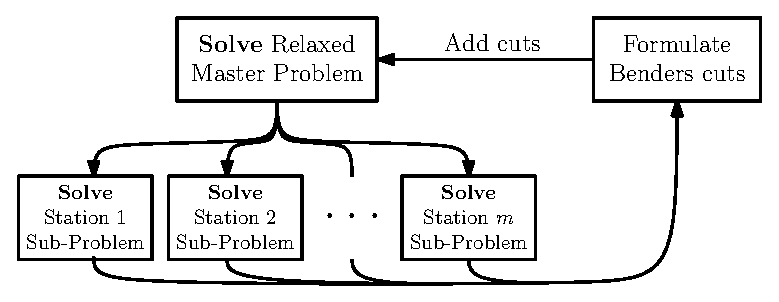
\includegraphics[width=0.9\textwidth]{images/ourHighLevelBenders.eps}
\end{figure}
\end{frame}

%------------------------------------------------
\begin{frame}
\frametitle{Solution Methodology: Overview}
% Talk about Chuffed and how good it is here
\begin{figure}
	\centering
	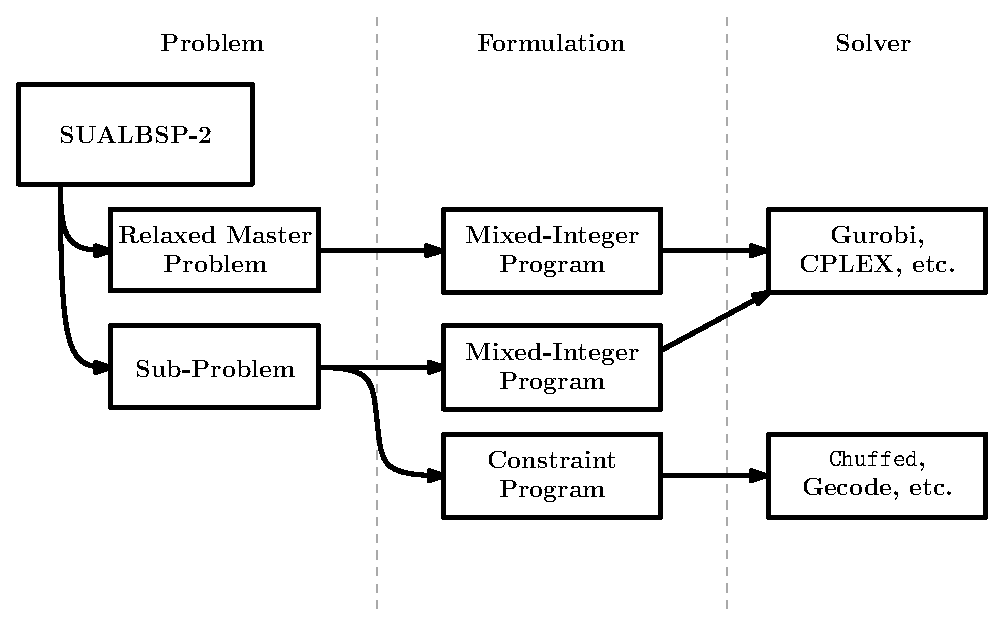
\includegraphics[width=0.95\textwidth]{images/bendersApproach.eps}
\end{figure}
\end{frame}

%------------------------------------------------
\begin{frame}
\frametitle{Master Problem Formulation}
Assignment problem $\Rightarrow$ Formulate a MIP, solve with Gurobi\pause
\begin{IEEEeqnarray}{rClCl}
	\IEEEeqnarraymulticol{3}{l}{\text{RMP($\mu$): Min } c^\mu} & \hspace{4mm} & \nonumber\\[2pt]
	\text{s.t. } & \hspace{4mm} & \sum_{k\in FS_i} x_{ik}^\mu = 1 & & \forall i \in V \nonumber\\[2pt]
	& & \sum_{k \in FS_i} k\cdot x_{ik}^\mu \leq \sum_{k \in FS_j} k\cdot x_{jk}^\mu & & \forall (i,j) \in E \nonumber\\[2pt]
	& & \sum_{i \in V} t_i \cdot x_{ik}^\mu \leq c^\mu & & \forall k \in K \nonumber\\[2pt]
	& & \mathcal{C}^\nu & & \nu \in \{1, 2,\ldots,\mu-1 \} \nonumber\\[2pt]
	& & \underline{c}^\mu\leq c^\mu \leq \bar{c}^\mu & &  \nonumber\\[2pt]
	& & x_{ik}^\mu\in\{0,1\} & & \forall i \in V,~ k \in FS_i \nonumber
\end{IEEEeqnarray}

\end{frame}

%------------------------------------------------
\begin{frame}
\frametitle{Sub-Problem Formulation}
\begin{itemize}
	\item `Kind of' similar to the asymmetric TSP $\Rightarrow$ highly combinatorial \vspace{2mm}\pause
\end{itemize}

\centering
\only<1>{
\includegraphics[width=0.4\textwidth]{images/tspSP-x.eps}}%
\only<2>{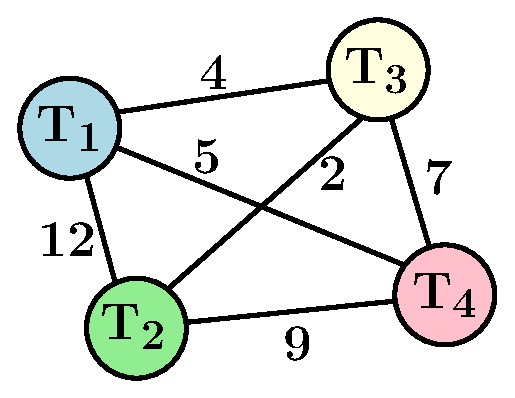
\includegraphics[width=0.4\textwidth]{images/tspSP-1.eps}}\pause%
\only<3>{\includegraphics[width=0.4\textwidth]{images/tspSP-2.eps}}\pause%
\only<4>{\includegraphics[width=0.4\textwidth]{images/tspSP-2.eps}}%
\only<5>{\includegraphics[width=0.4\textwidth]{images/tspSP-2.eps}}%

\begin{itemize}
	\item Possible approaches \vspace{2mm}
	\begin{itemize}
		\item Mixed-Integer Problem\vspace{1mm}
		\item Constraint Problem\vspace{1mm}
		\item Travelling Salesperson Problem (requires some adaptation)\vspace{1mm}\pause
		\begin{itemize}
			\item Pro: Use dedicated TSP solvers (Concorde, {\tt tsp\_solve} etc.)
			\item Con: Leads to multiplying number of tasks by $2n^2$ $\Rightarrow$ Did not explore
		\end{itemize}
	\end{itemize}
\end{itemize}
\end{frame}


%------------------------------------------------
\begin{frame}
\frametitle{Sub-Problem: Mixed Integer Program}
\vspace{-0.8cm}
\begin{IEEEeqnarray}{rClCl}
	\IEEEeqnarraymulticol{3}{l}{\text{SP-MIP($\mu$): Min } l_k^\mu} & \hspace{4mm} & \nonumber\\[2pt]
	\text{s.t. } & \hspace{4mm} & \sum_{j \in F_i^\phi} y_{ij} + \sum_{j \in F_i^\beta} z_{ij} = 1 & & \forall i \in V_k^\mu \nonumber\\[2pt]
	& & \sum_{i \in P_j^\phi} y_{ij} + \sum_{i \in P_j^\beta} z_{ij} = 1 & & \forall j \in V_k^\mu \nonumber\\[2pt]
	& & \sum_{i\in V_k^\mu} \sum_{j\in F_i^\beta} z_{ij} =1 & &  \nonumber\\[2pt]
	& & s_i + t_i + \phi_{ij}\cdot y_{ij} \leq s_j & & \forall (i,j) \in E_k^\mu \nonumber\\[2pt]
	& & s_i + t_i + \phi_{ij} \leq s_j + {\color{red} M}(1-y_{ij}) & & \forall i\in V_k^\mu,~ j \in F_i^\phi  \nonumber\\[2pt]
	& & s_i + t_i + \sum_{j\in F_i^\beta}\beta_{ij}\cdot z_{ij} \leq l_k^\mu & & \forall i\in V_k^\mu \nonumber\\[2pt]
	& & l_k^\mu \geq 0,~s_i \geq 0 & & \forall i \in V_k^\mu \nonumber\\[2pt]
	& & y_{ij}^\mu~(z_{ij}^\mu)\in\{0,1\} & & \forall i \in V_k^\mu,~ j \in F_i^\phi(F_i^\beta) \nonumber
\end{IEEEeqnarray}
\end{frame}

%------------------------------------------------
\begin{frame}
\frametitle{Sub-Problem: Constraint Program}
\begin{itemize}
	\item Contraint Programming handles scheduling problems well\vspace{2mm}\pause
	\item Expressive nature of CP removes need for big-$M$ constraints\vspace{2mm}\pause
	\item {\tt Chuffed} is a state-of-the-art solver for many scheduling problems\vspace{2mm}\pause
	\item `Learning' solver which combines\vspace{2mm}
	\begin{itemize}
		% \item Nogood learning\vspace{1mm}
		\item Lazy clause generation\vspace{1mm}
		\item Boolean satisfiability solving
	\end{itemize}
\end{itemize}
\end{frame}

%------------------------------------------------
\begin{frame}
\frametitle{CP Solver Chuffed: Global Constraints}

\begin{itemize}
	\item First main advantage of CP\vspace{1mm}
	\item Capture common combinatorial structures across problems\vspace{1mm}
	\item Provide effective propagation for CP solvers\vspace{2mm}\pause
	\item Some include:\vspace{2mm}
	\begin{itemize}
		\item {\tt knapsack}()\vspace{1mm}
		\item {\tt disjunctive}()\vspace{1mm}
		\item {\tt cumulative}()\vspace{1mm}
		\item {\tt bin\_packing}()\vspace{1mm}
		\item \small{\tt int\_set\_channel}()\vspace{1.5mm}
		\item \footnotesize{\tt diffn}()\vspace{1mm}
		\item \scriptsize{\tt geost}()\vspace{2mm}
		\item \tiny{\tt all\_different}()\vspace{1mm}
		\item $\qquad\vdots$
	\end{itemize}
\end{itemize}
\end{frame}

%------------------------------------------------
\begin{frame}
\frametitle{CP Solver Chuffed: Search Strategy}
\begin{itemize}
	\item Second main advantage of CP\vspace{1mm}
	\item Combinatorial problem $\Rightarrow$ Constant battle against huge solution space\vspace{1mm}\pause
	\item Search strategies are a powerful weapon here\pause
\end{itemize}
\vspace{3mm}
{\tt Chuffed}'s search language:\vspace{2mm}\pause
\begin{itemize}
	\item Basic searches\vspace{1mm}
	\begin{itemize}
		\item Integers: {\tt int\_search}\vspace{1mm}
		\item Booleans: {\tt bool\_search}\vspace{2mm}\pause
	\end{itemize}
	\item Compositional searches\vspace{1mm}
	\begin{itemize}
		\item Sequential: {\tt seq\_search}\vspace{1mm}\pause
		\item {\color{red} new!} Priority: {\tt priority\_search}
	\end{itemize}
\end{itemize}
\end{frame}


%------------------------------------------------
\begin{frame}
\frametitle{Benders Cuts}
\begin{itemize}
	\item Communicate information from sub-problems to master problem\vspace{2mm}
	\item Richer information leads to faster convergence\vspace{2mm}\pause
	\item We proposed a range of cutting procedures:
\end{itemize}
\begin{table}[tpb]
	\def\arraystretch{1.2}
	\setlength{\tabcolsep}{3mm}
	\centering
	\begin{tabular}{ll}
		% \multicolumn{2}{l}{}\\[3mm]\pause
		\toprule
		Feasibility Cuts & Optimality Cuts \\\midrule\midrule
		Nogood cut & Logic cut\\
		 & Inference cut \#1 (simple)\\
		 & Inference cut \#2 (smarter)\\
		 & Inference cut \#3 (smartest)\\
		 & Global cut/bound\\
		\bottomrule
	\end{tabular}
\end{table}
\end{frame}

%------------------------------------------------
\begin{frame}
\frametitle{Benders Cuts: Inference Cut Example}
% Inference cut \#3:
% \begin{IEEEeqnarray}{rCcCl}
% 	&\hspace{4mm}& l_k^\nu -\sum_{i\in V_k^\nu} \bar{B}_{ik}^\nu(1-x_{ik}^\mu) + \sum_{i\in V\setminus V_k^\nu} b_{ik}^\nu \cdot x_{ik}^\mu \leq c^\mu &\hspace{4mm}& \nonumber	
% \end{IEEEeqnarray}\pause
Inference cut \#1 (simple):
\begin{IEEEeqnarray}{rCcCl}
	&\hspace{4mm}& l_k^\nu -M \sum_{i\in V_k^\nu} (1-x_{ik}^\mu) \leq c^\mu &\hspace{4mm}& \nonumber	
\end{IEEEeqnarray}
\vspace{1mm}
\begin{itemize}
	\item If same assignment as before $\Rightarrow$ Lower bound on cycle time\vspace{2mm}\pause
\end{itemize}
Inference cut \#3 (smartest):
\begin{IEEEeqnarray}{rCcCl}
	&\hspace{4mm}& l_k^\nu -\sum_{i\in V_k^\nu} B_{ik}^\nu(1-x_{ik}^\mu) + \sum_{i\in V\setminus V_k^\nu} b_{ik}^\nu \cdot x_{ik}^\mu \leq c^\mu &\hspace{4mm}& \nonumber	
\end{IEEEeqnarray}
\vspace{1mm}
\begin{itemize}
	\item If {\it similar} assignment as before $\Rightarrow$ Lower bound on cycle time\vspace{2mm}
\end{itemize}
\end{frame}

%------------------------------------------------
\begin{frame}
\Huge{\centerline{Results}}
\end{frame}

%------------------------------------------------
\begin{frame}
\frametitle{Benders Results: Sub-Problem Formulations}
\begin{itemize}
	\item Medium sized instances\vspace{1mm}
	\item Time limit: 30 minutes on each instance
\end{itemize}
\begin{table}
	\centering
	\begin{tabular}{ccrrrr}
		\toprule
		\#Tasks & Type & \#SP Nodes & \%Gap & \%Opt. & SP Runtime(s) \\\midrule\midrule
		25--30 & SP-MIP{} & 639k & 11.7 & 82.1 & 226.2 \\
		 & SP-CP{} & 1,692k & 13.0 & {\bf 83.9} & 229.4 \\
		\bottomrule
	\end{tabular}
\end{table}
\end{frame}

%------------------------------------------------
\begin{frame}
\frametitle{Benders Results: Comparison with MIPs}
\begin{itemize}
	\item All 3 data sets\vspace{1mm}
	\item Time limit: 30 minutes on each instance
\end{itemize}
\begin{table}
	\setlength{\tabcolsep}{0.2em}
	\centering
	\small
	\begin{tabular}{crrrrrrrrr}
		\toprule
		& \multicolumn{3}{c}{Benders} & \multicolumn{3}{c}{MIP-1} & \multicolumn{3}{c}{MIP-2}  \\
		 \cmidrule(lr){2-4} \cmidrule(lr){5-7} \cmidrule(lr){8-10}
		\#Tasks & \%Gap &\%NoSol. &  \%Opt. & \%Gap & \%NoSol. & \%Opt. & \%Gap & \%NoSol. & \%Opt. \\\midrule\midrule
		7--21 & 0.0 & 0.0 & {\color{red} 100.0} & 0.1 & 0.0 & {\color{red} 93.5} & 1.6 & 0.0 & {\color{red} 77.8} \\
		25--30 & 13.0 & 0.0 & {\color{red} 83.9} & 13.8 & 0.0 & {\color{red} 0.0} & 18.0 & 25.0 & {\color{red} 0.0} \\
		32--58 & 35.8 & 0.0 & {\color{red} 32.4} & 19.6 & 5.1 & {\color{red} 3.9} & 10.1 & 61.9 & {\color{red} 0.0} \\
		\bottomrule
	\end{tabular}
\end{table}\pause
\begin{itemize}
	\item Solved the small instances in 0.1 seconds on average
	\item ``...more efficient exact methods.'' \pause Done $\checkmark$
\end{itemize}
\end{frame}

%------------------------------------------------
\begin{frame}
\frametitle{Benders Results: Runtime Distribution}
\begin{itemize}
	\item All 3 data sets\vspace{1mm}
	\item Time limit: 30 minutes on each instance
\end{itemize}
\begin{table}
	\centering
	\begin{tabular}{crrrr}
		\toprule
		\#Tasks & \# Iters. & \# Cuts & Master Runtime (s) & SP Runtime(s) \\\midrule\midrule
		7--21 & 3 & 9 & 0.03 (27.3\%) & 0.08 (72.7\%) \\
		25--30 & 71 & 262 & 269.9 (54.1\%) & 229.4 (45.9\%) \\
		32--58 & 21 & 113 & 832.5 (65.4\%) & 440.9 (34.6\%) \\
		\bottomrule
	\end{tabular}
\end{table}
\end{frame}

%------------------------------------------------
\begin{frame}
\frametitle{Conclusion}
\begin{itemize}
	\item Proposed a logic-based Benders decomposition framework\vspace{2mm}
	\begin{itemize}
		\item Together with some Benders cuts\vspace{3mm}
	\end{itemize}\pause
	\item Optimally solved 257 of the 396 instances in 30 minute time limit\vspace{2mm}
	\begin{itemize}
		\item {\color{red} Closed 149 open instances}
	\end{itemize}
\end{itemize}
\end{frame}


%------------------------------------------------
\begin{frame}
\frametitle{Future Work}
% \begin{figure}
% 	\centering
% 	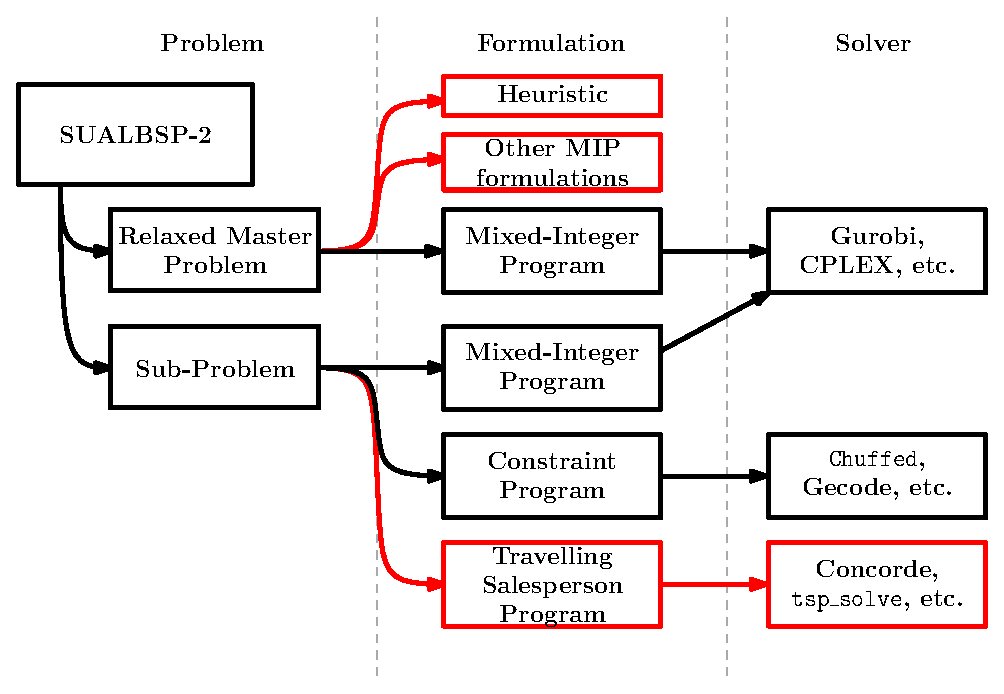
\includegraphics[width=0.95\textwidth]{images/futureBendersApproach-1.eps}
% \end{figure}
\centering
\only<1>{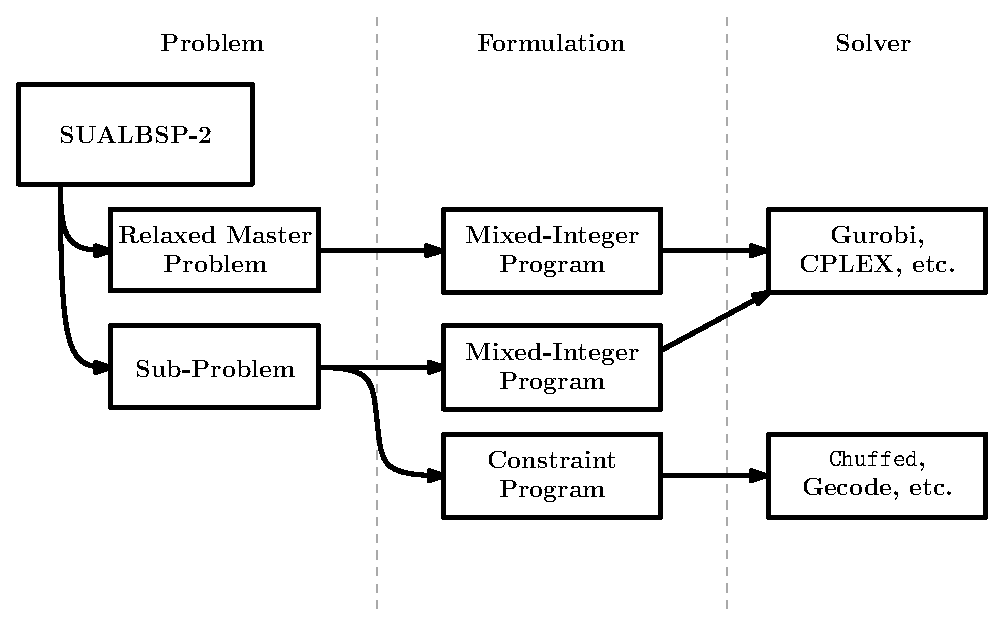
\includegraphics[width=0.95\textwidth]{images/bendersApproach.eps}}%
\only<2>{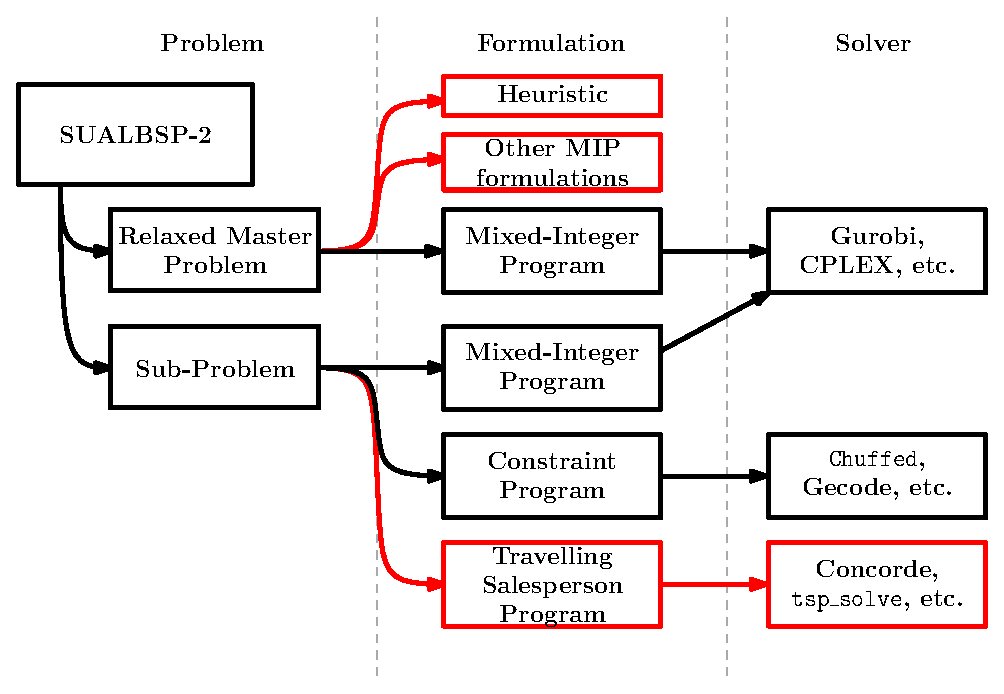
\includegraphics[width=0.95\textwidth]{images/futureBendersApproach-1.eps}}%
\only<3>{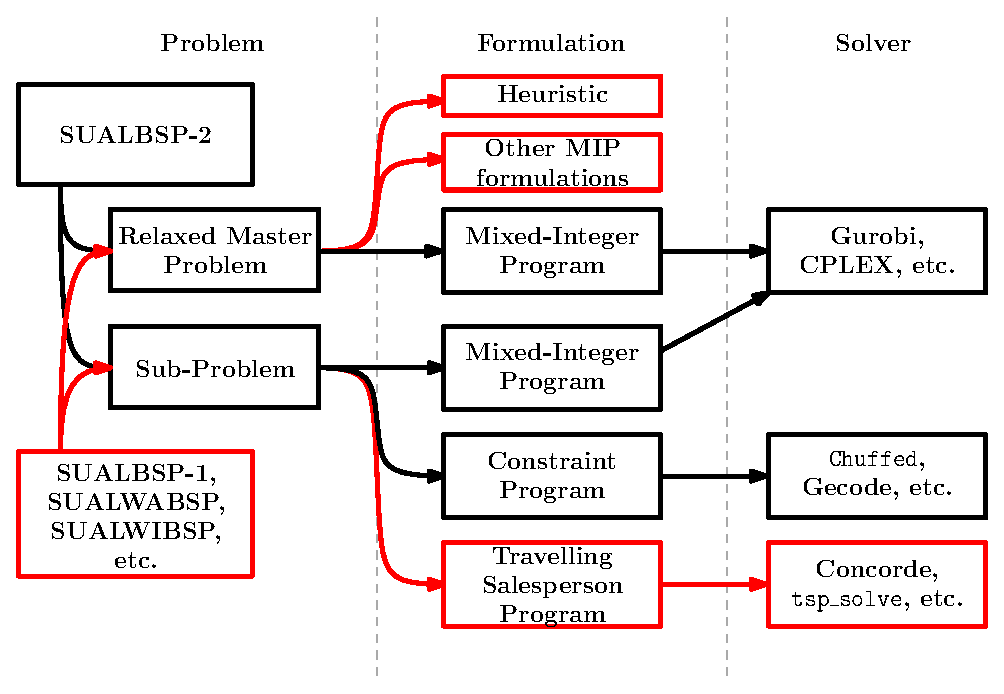
\includegraphics[width=0.95\textwidth]{images/futureBendersApproach-2.eps}}%
\end{frame}



%------------------------------------------------

\begin{frame}
\Huge{\centerline{Thanks for listening!}}
\vspace{2cm}
\large{\centerline{Any questions?}}
\end{frame}

%----------------------------------------------------------------------------------------

\end{document}